\documentclass[12pt,a4paper]{article}

% ── Packages ──────────────────────────────────────────────────────────────────
\usepackage[utf8]{inputenc}
\usepackage[T1]{fontenc}
\usepackage{lmodern}
\usepackage[margin=2.5cm]{geometry}
\usepackage{titlesec}
\usepackage{hyperref}
\usepackage{xcolor}
\usepackage{booktabs}
\usepackage{longtable}
\usepackage{array}
\usepackage{enumitem}
\usepackage{graphicx}
\usepackage{float}
\usepackage{listings}
\usepackage{fancyhdr}
\usepackage{tocloft}
\usepackage{caption}
\usepackage{subcaption}
\usepackage{mdframed}
\usepackage{amsmath}
\usepackage{microtype}
\usepackage{parskip}

% ── Colours ───────────────────────────────────────────────────────────────────
\definecolor{accentblue}{RGB}{30,90,160}
\definecolor{codegreen}{RGB}{0,128,0}
\definecolor{codegray}{RGB}{128,128,128}
\definecolor{codepurple}{RGB}{120,0,120}
\definecolor{backcolour}{RGB}{248,248,248}
\definecolor{adrcolor}{RGB}{245,247,250}

% ── Listings style ────────────────────────────────────────────────────────────
\lstdefinestyle{mystyle}{
  backgroundcolor=\color{backcolour},
  commentstyle=\color{codegreen},
  keywordstyle=\color{accentblue}\bfseries,
  numberstyle=\tiny\color{codegray},
  stringstyle=\color{codepurple},
  basicstyle=\ttfamily\small,
  breakatwhitespace=false,
  breaklines=true,
  captionpos=b,
  keepspaces=true,
  numbers=left,
  numbersep=5pt,
  showspaces=false,
  showstringspaces=false,
  showtabs=false,
  tabsize=2,
  frame=single,
  rulecolor=\color{gray!30}
}
\lstset{style=mystyle}

% ── Headers / Footers ─────────────────────────────────────────────────────────
\pagestyle{fancy}
\fancyhf{}
\fancyhead[L]{\small\textit{AlumniConnect -- Technical Architecture Report}}
\fancyhead[R]{\small\textit{S26CS6.401 -- Team 40}}
\fancyfoot[C]{\thepage}
\renewcommand{\headrulewidth}{0.4pt}

% ── Section formatting ────────────────────────────────────────────────────────
\titleformat{\section}{\large\bfseries\color{accentblue}}{\thesection}{1em}{}[\titlerule]
\titleformat{\subsection}{\normalsize\bfseries\color{accentblue!80}}{\thesubsection}{1em}{}
\titleformat{\subsubsection}{\normalsize\bfseries}{\thesubsubsection}{1em}{}

% ── ADR box ───────────────────────────────────────────────────────────────────
\newmdenv[
  backgroundcolor=adrcolor,
  linecolor=accentblue,
  linewidth=1.5pt,
  leftline=true,
  rightline=false,
  topline=false,
  bottomline=false,
  innerleftmargin=12pt,
  innerrightmargin=10pt,
  innertopmargin=8pt,
  innerbottommargin=8pt
]{adrbox}

% ── Hyperref setup ────────────────────────────────────────────────────────────
\hypersetup{
  colorlinks=true,
  linkcolor=accentblue,
  urlcolor=accentblue,
  citecolor=accentblue,
  pdftitle={AlumniConnect -- Technical Architecture Report},
  pdfauthor={Team 40},
}

% ══════════════════════════════════════════════════════════════════════════════
\begin{document}

% ── Title Page ────────────────────────────────────────────────────────────────
\begin{titlepage}
  \centering
  \vspace*{2cm}
  {\Large\bfseries Software Engineering CS6.401 --- Spring 2026}\\[0.4cm]
  {\huge\bfseries Phase-3 Project Report}\\[1.2cm]
  {\Large\bfseries\color{accentblue} AlumniConnect Mentorship Platform}\\[1.2cm]
  \rule{\textwidth}{0.5pt}\\[1cm]
  {\Large \textbf{Team Number: 40}}\\[0.8cm]
  {\large \textbf{Repository:} \url{https://github.com/Dhanushdevireddy/AlumniConnect}}\\[0.8cm]
  
  
  \renewcommand{\arraystretch}{1.5}
  \begin{tabular}{ll}
    \textbf{Name} & \textbf{Roll Number} \\
    Sriram Metla & 2024201059 \\
    Dhanush Devireddy & 2024201028 \\
    Chandana Pappula & 2024201060 \\
    Yaswanth Chandaluri & 2024201045 \\
    AdhiVishnu Modapu & 2024202028 \\
  \end{tabular}
  
  \vfill
\end{titlepage}

% ── Table of Contents ─────────────────────────────────────────────────────────
\tableofcontents
\newpage

\section*{System Overview}
\addcontentsline{toc}{section}{System Overview}

AlumniConnect is a comprehensive web platform designed to bridge the structural gap between university students seeking career mentorship and alumni willing to provide it. The platform delivers structured, on-demand mentorship through a rich feature set, including a ranked alumni directory, a state-machine-governed mentoring request lifecycle, persistent real-time chat, and collaborative session scheduling. The system is built as a layered monolithic architecture, optimizing for development velocity and deployment simplicity while retaining high scalability through strategic component decoupling.

\begin{figure}[H]
  \centering
  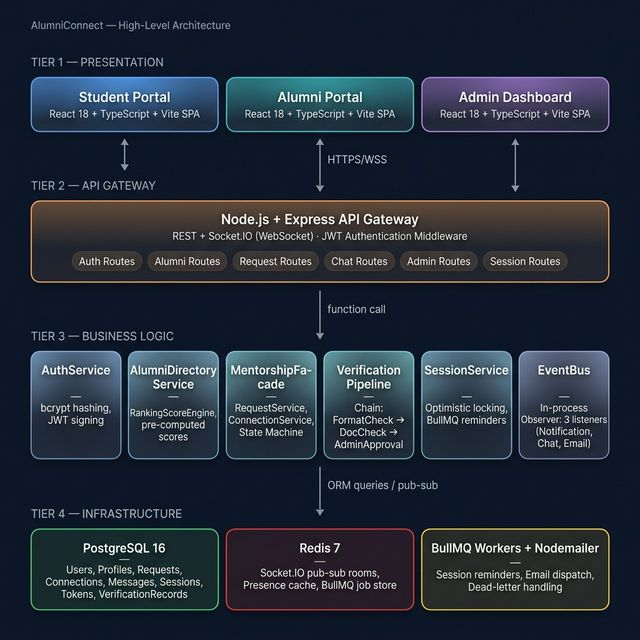
\includegraphics[width=\textwidth]{alumniconnect_hld.png}
  \caption{AlumniConnect High-Level Architecture}
\end{figure}

\begin{figure}[H]
  \centering
  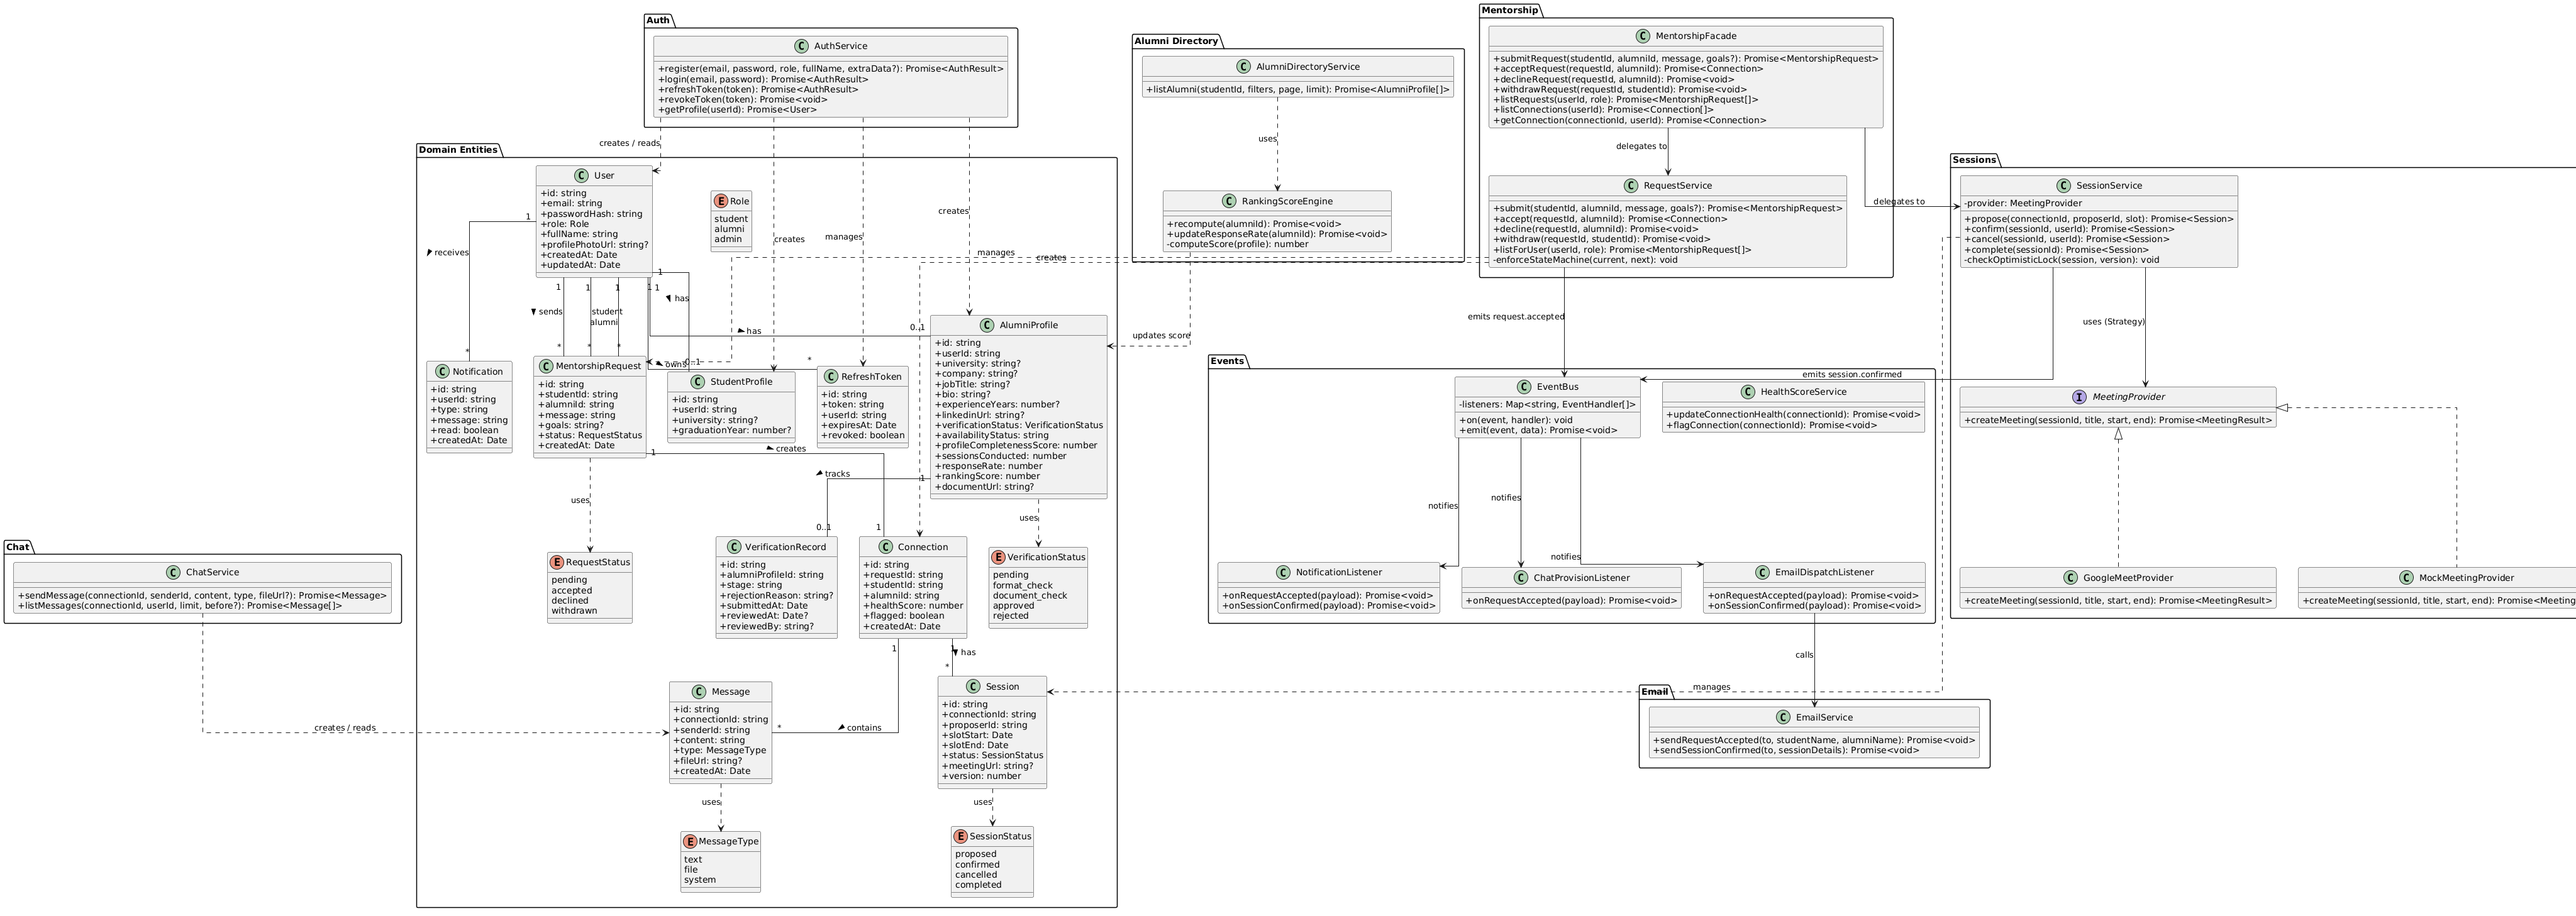
\includegraphics[width=1.0\textwidth]{class_diagram.png}
  \caption{AlumniConnect Class Diagram detailing domain entities and service patterns}
\end{figure}

\subsection*{Architecture Models (C4)}
\addcontentsline{toc}{subsection}{Architecture Models (C4)}

To further specify the system boundaries and component interactions, the following C4 models have been defined:

\begin{figure}[H]
  \centering
  \begin{subfigure}[b]{0.32\textwidth}
    \centering
    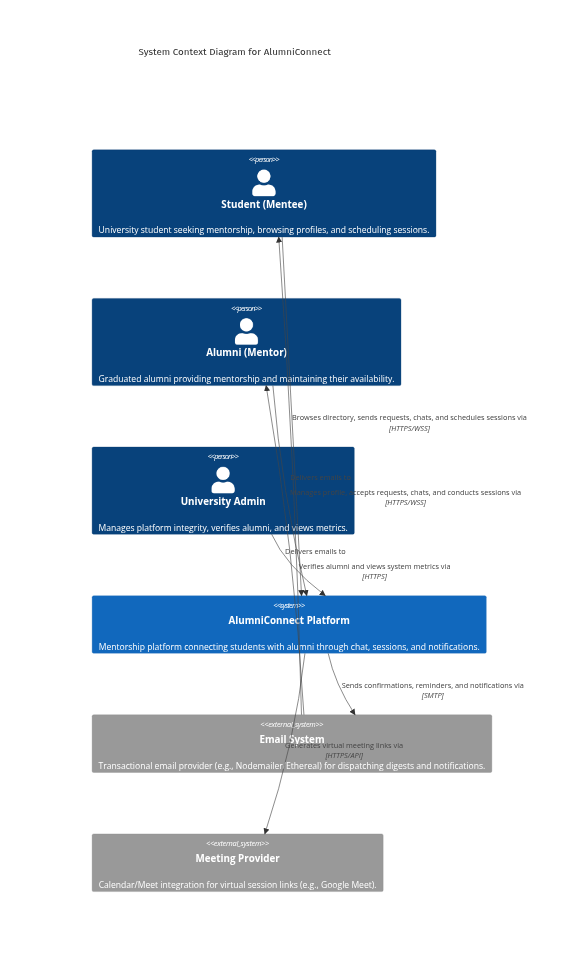
\includegraphics[width=\textwidth]{c4_context.png}
    \caption{Level 1: System Context}
  \end{subfigure}
  \hfill
  \begin{subfigure}[b]{0.32\textwidth}
    \centering
    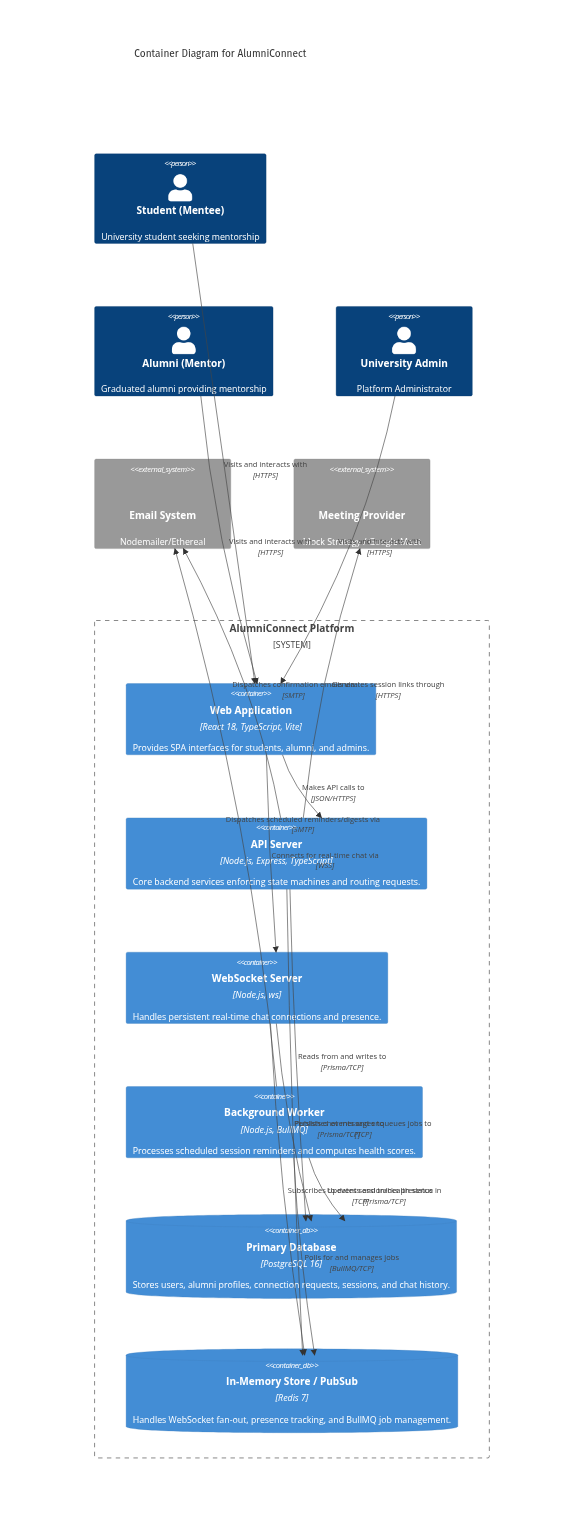
\includegraphics[width=\textwidth]{c4_container.png}
    \caption{Level 2: Container}
  \end{subfigure}
  \hfill
  \begin{subfigure}[b]{0.32\textwidth}
    \centering
    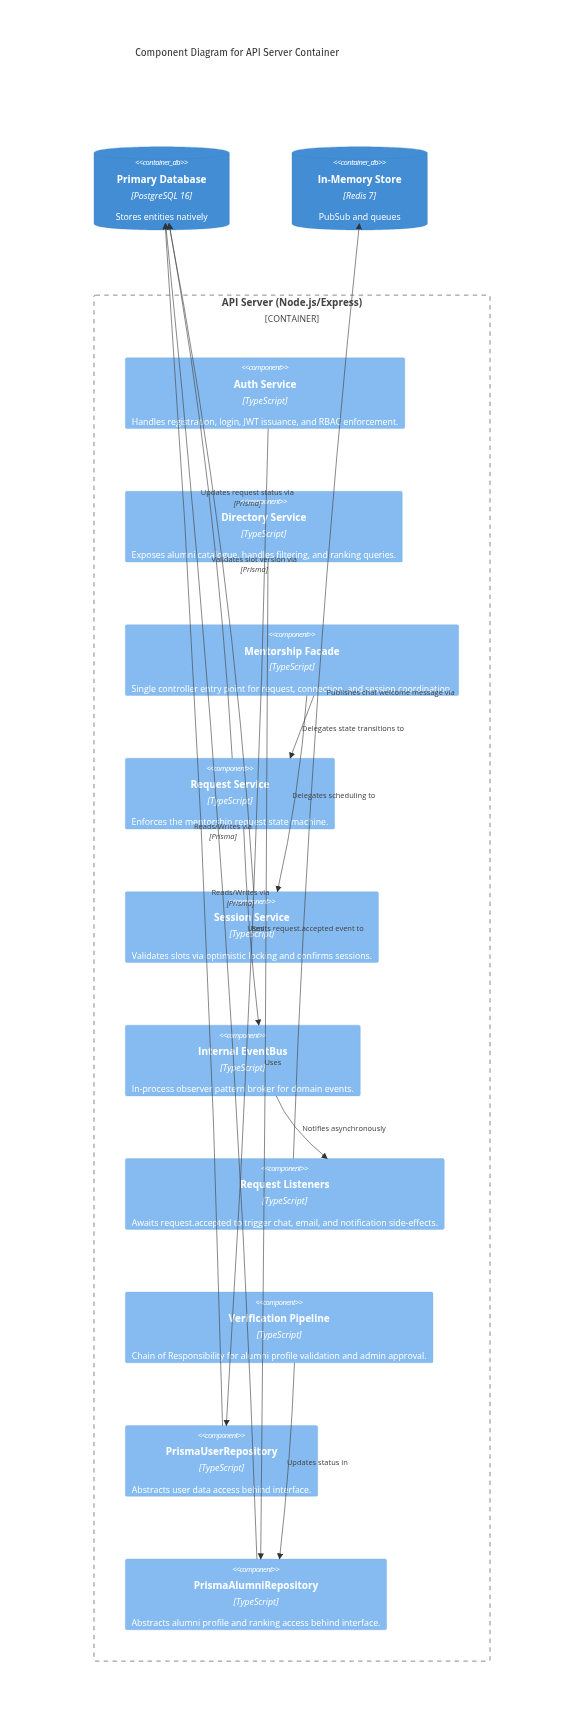
\includegraphics[width=\textwidth]{c4_component.png}
    \caption{Level 3: Component}
  \end{subfigure}
  \caption{C4 Architecture Models (Levels 1--3) for AlumniConnect}
\end{figure}

\section*{System Flow}
\addcontentsline{toc}{section}{System Flow}

At its core, AlumniConnect operates through well-defined event-driven flows that decouple user actions from asynchronous side effects. The primary request lifecycle bridges the gap between students and alumni via an explicitly enforced state machine. Upon crucial state transitions---such as the acceptance of a mentorship request---the system utilizes an internal Observer pattern to seamlessly trigger downstream provisions. This guarantees that critical side-effects, such as real-time chat thread creation, session enablement, and multi-channel email dispatch, occur reliably without blocking the primary interaction cycle.

\begin{figure}[H]
  \centering
  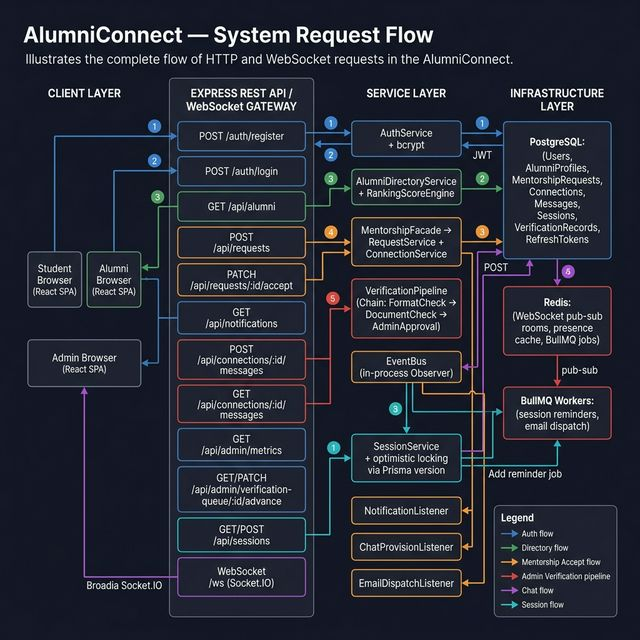
\includegraphics[width=1.0\textwidth]{alumniconnect_request_flow.png}
  \caption{AlumniConnect complete System Request Flow}
\end{figure}

\newpage



% ══════════════════════════════════════════════════════════════════════════════
%  TASK 1 -- REQUIREMENTS AND SUBSYSTEMS
% ══════════════════════════════════════════════════════════════════════════════
\section{Task 1: Requirements and Subsystems}

\subsection{Functional Requirements}

The following functional requirements were identified and are architecturally significant because they each impose distinct structural constraints on the system.

\begin{longtable}{@{}p{1.4cm} p{3.8cm} p{7.5cm}@{}}
\toprule
\textbf{ID} & \textbf{Feature} & \textbf{Description} \\
\midrule
\endhead
FR1 & Alumni Directory \& Ranked Matching & Queryable alumni catalogue with server-side filtering by domain, company, and availability. Profiles are ranked by a weighted scoring function over four signals: \textit{profile completeness} (25\%), \textit{sessions conducted} (30\%), \textit{response rate} (30\%), and \textit{domain tag coverage} (15\%). Scores are recomputed incrementally on each interaction event and persisted for fast read access. \\[4pt]
FR2 & Mentorship Request System & Students submit personalised requests to available mentors. Requests transition through an explicit state machine (\texttt{Pending} $\to$ \texttt{Accepted} $|$ \texttt{Declined} $|$ \texttt{Withdrawn}) enforced at the service layer. On acceptance, the Observer pattern fires a decoupled event pipeline: connection record creation, chat thread provisioning, notification dispatch, and dual email delivery. \\[4pt]
FR3 & Real-Time Chat & Each accepted connection opens a dedicated persistent WebSocket channel supporting text and binary PDF uploads. Messages are durably written to PostgreSQL. A pub-sub mechanism (Redis) fans out messages across server instances. A presence-tracking service maintains live online/offline state per connection. \\[4pt]
FR4 & Session Scheduling & Either party proposes a time slot. The scheduling service validates the slot against existing bookings using optimistic locking to prevent conflicts. On mutual confirmation, the calendar integration generates a virtual meeting link and dispatches invites. A BullMQ job scheduler enqueues reminder notifications at T$-$24\,h and T$-$1\,h. \\[4pt]
FR5 & Admin Dashboard & Alumni registrations enter a Chain of Responsibility verification pipeline (format check $\to$ document validation $\to$ admin approval). Approved profiles become discoverable. Admins manage domain taxonomy and view aggregated platform metrics. \\[4pt]
FR6 & Smart Notification Digest & Pending events per user are aggregated by a scheduled digest pipeline. Runs at a user-configured cadence (daily or weekly), compiling a structured per-user feed into a single batched email. \\[4pt]
FR7 & Connection Health Score & A time-decaying engagement score (0--1) computed per active connection from message frequency (40\%), session attendance rate (35\%), and inter-message response latency (25\%), multiplied by a recency decay factor. Connections below a staleness threshold of 0.35 are automatically flagged and re-engagement nudges are dispatched. \\
\bottomrule
\end{longtable}

\subsubsection{Architecturally Significant Requirements}

\begin{itemize}[leftmargin=*]
  \item \textbf{FR1 -- Ranked Matching:} Drives the separation of the \textit{scoring engine} from the query path; scores must be pre-computed to satisfy the sub-500\,ms directory query requirement.
  \item \textbf{FR2 -- State Machine:} Requires an explicit service-layer enforcement layer (not only DB constraints) to prevent invalid transitions (e.g., accepting an already-withdrawn request), introducing the \textit{MentorshipFacade} subsystem.
  \item \textbf{FR3 -- Real-Time Chat:} Mandates a horizontally scalable WebSocket tier backed by Redis pub-sub; cannot be served over plain HTTP.
  \item \textbf{FR5 -- Verification Pipeline:} Requires a pluggable Chain of Responsibility handler so that new verification stages can be inserted without modifying existing handlers.
  \item \textbf{FR7 -- Health Score:} Requires a background computation job with rolling time-window semantics, decoupled from the request-response cycle.
\end{itemize}

\subsection{Non-Functional Requirements}

\begin{longtable}{@{}p{2.8cm} p{10cm}@{}}
\toprule
\textbf{Category} & \textbf{Quantified Requirement} \\
\midrule
\endhead
Performance & API p95 response $<$ 200\,ms. Chat message delivery $<$ 100\,ms end-to-end. Ranked directory queries $<$ 500\,ms over 10,000 profiles. \\[4pt]
Scalability & WebSocket tier scales horizontally via Redis pub-sub fan-out across stateless instances. Chat, notification, and job-scheduler services are independently deployable. \\[4pt]
Availability & Uptime $\geq$ 99.5\%. WebSocket auto-reconnects within 5\,s without message loss. BullMQ jobs persist across restarts and re-enqueue on recovery. \\[4pt]
Reliability & No message lost on disconnect/reconnect. Concurrent slot requests serialised via optimistic locking. Critical state-mutation endpoints are idempotent. \\[4pt]
Security & JWT access tokens expire in 24\,h with refresh-token rotation. RBAC enforced on every protected route. Alumni invisible until admin-verified. All traffic over HTTPS. \\[4pt]
Modifiability & New meeting provider: $\leq$ 1 interface change. New notification channel: zero lifecycle-service changes. New ranking signal: injectable without modifying the scoring engine. \\
\bottomrule
\end{longtable}

\subsection{Subsystem Overview}

The system is decomposed into eight primary subsystems, each with a well-defined responsibility boundary.

\begin{longtable}{@{}p{3.5cm} p{9.2cm}@{}}
\toprule
\textbf{Subsystem} & \textbf{Role \& Functionality} \\
\midrule
\endhead
\textbf{Auth Service} & Handles user registration and login. Issues JWT access tokens and manages refresh-token rotation. Enforces role-based guards (Student / Alumni / Admin) at the API boundary via Express middleware. \\[4pt]
\textbf{Directory Service} & Exposes the alumni catalogue with server-side filtering (domain, company, availability). Delegates ranking reads to the pre-computed \texttt{rankingScore} column; never recomputes at query time. \\[4pt]
\textbf{Mentorship Service} & Facade over the request state machine, connection creation, and chat thread provisioning. Enforces valid state transitions and emits the \texttt{request.accepted} domain event via the internal EventBus. \\[4pt]
\textbf{Chat Service} & Manages WebSocket connection lifecycle, message persistence, and file uploads. Publishes messages to a Redis pub-sub channel so all server instances receive and forward them. Maintains per-connection presence state in Redis. \\[4pt]
\textbf{Session Service} & Validates proposed time slots against existing bookings using optimistic locking (\texttt{version} column). Confirms sessions, invokes the Meeting Provider, and enqueues BullMQ reminder jobs. \\[4pt]
\textbf{Notification Service} & Stores notification events per user. Supports per-notification read/unread toggle and a batched mark-all-read endpoint. The digest pipeline aggregates unread events into structured emails at the configured cadence. \\[4pt]
\textbf{Health Score Service} & Runs on a BullMQ schedule, computing a composite engagement score per connection over a rolling 30-day window. Flags low-health connections and dispatches re-engagement nudges. \\[4pt]
\textbf{Verification Pipeline} & Implements the Chain of Responsibility pattern across three stages (format check, document check, admin approval). Each handler advances the verification record or short-circuits with rejection. \\
\bottomrule
\end{longtable}

\newpage

% ══════════════════════════════════════════════════════════════════════════════
%  TASK 2 -- ARCHITECTURE FRAMEWORK
% ══════════════════════════════════════════════════════════════════════════════
\section{Task 2: Architecture Framework}

\subsection{Stakeholder Identification (IEEE 42010)}

Following the IEEE 42010:2011 standard for Architecture Description, stakeholders, their concerns, and the viewpoints that address those concerns are identified below.

\begin{longtable}{@{}p{2.8cm} p{3.8cm} p{5.6cm}@{}}
\toprule
\textbf{Stakeholder} & \textbf{Concerns} & \textbf{Viewpoint / View} \\
\midrule
\endhead
\textbf{Students (Mentees)} & Discovery of relevant alumni; request tracking; real-time chat access; session continuity. & Functional View -- Alumni directory, request lifecycle, chat and session flows. \\[4pt]
\textbf{Alumni (Mentors)} & Notification of incoming requests; availability management; privacy until verified. & Functional View + Security View -- Profile visibility gate; RBAC enforcement. \\[4pt]
\textbf{University Admin} & Platform integrity; alumni legitimacy; domain taxonomy control; engagement metrics. & Process View -- Verification pipeline; Admin dashboard metrics endpoint. \\[4pt]
\textbf{Development Team} & Maintainability; testability; horizontal scalability; low coupling between services. & Development View -- Service decomposition, EventBus, Repository interfaces. \\[4pt]
\textbf{Operations Team} & System availability; crash recovery; job persistence; deployability. & Deployment View -- Docker containers, BullMQ persistence, Redis pub-sub. \\[4pt]
\textbf{End Users (general)} & Response time; data privacy; browser-compatible interface. & Quality View -- NFR benchmarks: p95 $<$ 200\,ms API, $<$ 100\,ms chat. \\
\bottomrule
\end{longtable}

\subsubsection{Viewpoint -- Functional View}
Addresses \textit{what} the system does. Represented by the subsystem decomposition in Section~1.3 and the functional requirement table in Section~1.1.

\subsubsection{Viewpoint -- Concurrency \& Process View}
Addresses parallel execution and synchronisation. Critical concerns: (i)~WebSocket fan-out via Redis, (ii)~BullMQ workers for background jobs, (iii)~optimistic locking for session slots.

\subsubsection{Viewpoint -- Development View}
Addresses code organisation and modifiability. The backend follows a \textit{services/routes/events} layering strategy; services are injected, not instantiated by routes, enabling unit testing without Express.

\subsubsection{Viewpoint -- Deployment View}
Addresses physical distribution. PostgreSQL and Redis run in Docker containers; the Node.js backend and React frontend are hosted as OS-level processes. The WebSocket server is co-located with the API server but logically separate.

\subsection{Architecture Decision Records (ADRs)}

ADRs are documented following the Nygard template.

\begin{adrbox}
\textbf{ADR-001: Observer Pattern via Internal EventBus for Request Acceptance}

\textbf{Status:} Accepted

\textbf{Context:} When a mentorship request is accepted, three downstream effects must occur: (1) a connection record must be created, (2) a chat thread must be provisioned, and (3) dual confirmation emails must be dispatched. Implementing all three sequentially inside \texttt{RequestService.accept()} would couple unrelated services and make each side-effect invisible to unit tests.

\textbf{Decision:} Introduce an in-process \texttt{EventBus} (Observer pattern). \texttt{RequestService.accept()} emits a \texttt{request.accepted} event after updating the request status. Independent listener classes (\texttt{RequestListeners.ts}) subscribe to this event and handle chat provisioning, notification creation, and email dispatch. Each listener runs inside \texttt{Promise.allSettled}, so a failure in one does not abort others.

\textbf{Consequences:}
\begin{itemize}[leftmargin=*,topsep=2pt]
  \item \textit{Positive:} New side-effects (e.g., Slack notification) can be added by registering a listener -- zero changes to \texttt{RequestService}.
  \item \textit{Negative:} In-process bus is not durable; listeners that crash after the event fires but before committing to the DB will silently lose work. Acceptable for v1 given no strict at-least-once delivery requirement.
\end{itemize}
\end{adrbox}

\vspace{0.8em}

\begin{adrbox}
\textbf{ADR-002: Strategy Pattern for the Meeting Provider}

\textbf{Status:} Accepted

\textbf{Context:} Session confirmation requires generating a virtual meeting link. Initially, only a mock Google Meet link is generated. Future versions may integrate Google Calendar API, Zoom API, or Microsoft Teams. Hard-coding the link generation inside \texttt{SessionService} would require service-layer changes on every provider switch.

\textbf{Decision:} Define a \texttt{MeetingProvider} interface with a single \texttt{generateLink(session)} method. A \texttt{MockMeetingProvider} implements this interface for the prototype. \texttt{SessionService} depends only on the interface, injected at startup. Switching to a real provider requires only implementing the interface and updating the DI binding.

\textbf{Consequences:}
\begin{itemize}[leftmargin=*,topsep=2pt]
  \item \textit{Positive:} Meets the modifiability NFR -- new meeting provider: $\leq$ 1 interface change.
  \item \textit{Positive:} \texttt{SessionService} remains testable without real calendar API credentials.
  \item \textit{Negative:} Adds one indirection layer; trivial overhead for developers unfamiliar with the pattern.
\end{itemize}
\end{adrbox}

\vspace{0.8em}

\begin{adrbox}
\textbf{ADR-003: Redis Pub-Sub for Horizontally Scalable WebSocket Chat}

\textbf{Status:} Accepted

\textbf{Context:} WebSocket connections are stateful and node-local. If the system runs multiple API server instances, a message sent to instance A cannot reach a client connected to instance B through in-memory broadcasting alone.

\textbf{Decision:} Each server instance subscribes to a Redis pub-sub channel (\texttt{chat:\{connectionId\}}). When a message is received from a WebSocket client, the server publishes it to Redis in addition to broadcasting locally. All instances receive the Redis message and forward it to any local clients subscribed to that connection.

\textbf{Consequences:}
\begin{itemize}[leftmargin=*,topsep=2pt]
  \item \textit{Positive:} WebSocket tier is horizontally scalable -- adding instances does not break cross-instance delivery.
  \item \textit{Positive:} Redis instance already required for session cache and presence tracking.
  \item \textit{Negative:} Redis becomes a single point of failure for chat delivery. Mitigated by Redis Sentinel or Cluster in production.
\end{itemize}
\end{adrbox}

\vspace{0.8em}

\begin{adrbox}
\textbf{ADR-004: Pre-Computed Ranking Score Persisted to Database Column}

\textbf{Status:} Accepted

\textbf{Context:} The alumni directory requires ranked results over up to 10,000 profiles within 500\,ms. Computing a weighted score across four signals at query time would require multiple joins and aggregate queries per HTTP request, making the p95 target unachievable.

\textbf{Decision:} Maintain a \texttt{ranking\_score} column on the \texttt{alumni\_profiles} table. The \texttt{RankingScoreEngine} recomputes this score only on relevant domain events (request accepted/declined, session completed). Directory queries sort by \texttt{ranking\_score DESC} with no runtime computation. A database index on \texttt{verification\_status + ranking\_score} covers the common filtered-and-sorted query pattern.

\textbf{Consequences:}
\begin{itemize}[leftmargin=*,topsep=2pt]
  \item \textit{Positive:} Directory queries are a simple indexed sort -- O(log N + K) time complexity.
  \item \textit{Negative:} Score is eventually consistent; an alumni's rank reflects their state as of the last interaction event, not at the precise moment of the query. Acceptable business trade-off.
\end{itemize}
\end{adrbox}

\newpage

% ══════════════════════════════════════════════════════════════════════════════
%  TASK 3 -- ARCHITECTURAL TACTICS AND PATTERNS
% ══════════════════════════════════════════════════════════════════════════════
\section{Task 3: Architectural Tactics and Patterns}

\subsection{Architectural Tactics}

\subsubsection{Tactic 1: Optimistic Locking for Concurrent Session Scheduling}

\textbf{NFR addressed:} Reliability -- ``Concurrent slot requests serialised to prevent double-booking.''

Session records carry a \texttt{version} integer. The \texttt{SessionService.confirm()} method executes:

\begin{lstlisting}[language=SQL, caption={Optimistic locking in session confirmation}]
UPDATE sessions
SET status = 'confirmed', meeting_link = $1,
    confirmed_at = NOW(), version = version + 1
WHERE id = $2 AND version = $3 AND status = 'proposed'
\end{lstlisting}

If two concurrent requests attempt to confirm the same session, only the one that reads the correct version will win; the other receives 0 affected rows and is returned a \texttt{409 Conflict} response. No explicit locks are held, preserving throughput.

\subsubsection{Tactic 2: Circuit-Isolated Event Handlers (Fault Isolation)}

\textbf{NFR addressed:} Reliability -- ``A failure in one side-effect must not abort others.''

All domain event handlers are invoked via \texttt{Promise.allSettled()}, which resolves even when individual handlers reject. This prevents email dispatch failure from rolling back chat thread provisioning, and vice versa. Each handler logs its own errors without propagating them.

\subsubsection{Tactic 3: Token-Based Authentication with Refresh Rotation (Security)}

\textbf{NFR addressed:} Security -- ``JWT tokens expire in 24\,h with refresh rotation.''

Short-lived access tokens (24\,h) are issued alongside long-lived refresh tokens stored in the database. On each refresh, the old token is revoked and a new pair is minted. Revoked tokens are permanently unusable; stolen refresh tokens can be invalidated server-side without expiring the user session entirely.

\subsubsection{Tactic 4: Incremental Score Computation (Performance)}

\textbf{NFR addressed:} Performance -- ``Ranked directory queries $<$ 500\,ms.''

Rather than recomputing ranking scores at query time, the \texttt{RankingScoreEngine} is invoked only on interaction-driven events (request accepted/declined, session completed). The computed score is persisted to a database column indexed alongside \texttt{verification\_status}. Directory reads are reduced to a single indexed \texttt{ORDER BY} scan.

\subsubsection{Tactic 5: BullMQ Persistent Job Queue (Availability)}

\textbf{NFR addressed:} Availability -- ``Scheduled jobs persist in the queue across restarts and re-enqueue on recovery.''

Session reminder notifications (T$-$24\,h and T$-$1\,h) and the nightly digest pipeline are enqueued as BullMQ jobs backed by Redis. If the server process restarts before a job fires, the job remains in the Redis queue and is picked up by the next worker process. BullMQ's \texttt{removeOnComplete} and \texttt{removeOnFail} settings are tuned to retain failed jobs for debugging.

\subsection{Design Patterns}

The following table summarises all five design patterns employed in AlumniConnect, their location in the codebase, and their primary purpose.

\begin{center}
\begin{tabular}{@{}p{2.5cm} p{4.8cm} p{5.3cm}@{}}
\toprule
\textbf{Pattern} & \textbf{Source File(s)} & \textbf{Purpose} \\
\midrule
Observer       & \texttt{EventBus.ts}, \texttt{RequestListeners.ts} & Decouple request acceptance from 3 downstream side-effects \\[3pt]
Strategy       & \texttt{MeetingProvider.ts} & Swap meeting-link provider without modifying \texttt{SessionService} \\[3pt]
Repository     & \texttt{PrismaUserRepository.ts}, \texttt{PrismaAlumniRepository.ts} & Isolate ORM from business logic; enable unit-testable services \\[3pt]
Facade         & \texttt{MentorshipFacade.ts} & Single controller entry-point over requests, connections, sessions \\[3pt]
Chain of Resp. & \texttt{VerificationPipeline.ts} & Multi-stage alumni verification with pluggable, short-circuiting handlers \\
\bottomrule
\end{tabular}
\end{center}

\subsubsection{Pattern 1: Observer (EventBus + Domain Listeners)}

\textbf{Intent:} Decouple the source of a domain event from all downstream effects, allowing handlers to be added, removed, or replaced independently.

\textbf{Implementation:} The \texttt{EventBus} class maintains a registry of typed handlers in \texttt{EventBus.ts}:

\begin{lstlisting}[language=JavaScript, caption={EventBus publish-subscribe in TypeScript}]
class EventBus {
  private listeners: Map<string, EventHandler[]> = new Map();

  on<T>(event: string, handler: EventHandler<T>): void {
    const handlers = this.listeners.get(event) ?? [];
    handlers.push(handler as EventHandler);
    this.listeners.set(event, handlers);
  }

  async emit<T>(event: string, data: T): Promise<void> {
    const handlers = this.listeners.get(event) ?? [];
    await Promise.allSettled(handlers.map(h => h(data)));
  }
}
\end{lstlisting}

On \texttt{request.accepted}, three independent listeners in \texttt{RequestListeners.ts} execute concurrently:

\begin{center}
\begin{tabular}{@{}p{4cm} p{8cm}@{}}
\toprule
\textbf{Listener} & \textbf{Responsibility} \\
\midrule
\texttt{NotificationListener} & Creates \texttt{request\_accepted} notification events for both parties \\
\texttt{ChatProvisionListener} & Inserts a system welcome message into the connection's chat thread \\
\texttt{EmailDispatchListener} & Sends confirmation emails to student and alumni via Nodemailer \\
\bottomrule
\end{tabular}
\end{center}

\textbf{Role in Architecture:} Central decoupling mechanism. Adding a new listener (e.g., Slack notification, analytics ping) requires zero modifications to \texttt{RequestService} or \texttt{MentorshipFacade}.

\vspace{1em}

\subsubsection{Pattern 2: Strategy (MeetingProvider)}

\textbf{Intent:} Define a family of interchangeable algorithms behind a common interface so that the algorithm can be swapped without modifying the code that uses it.

\textbf{Implementation:}

\begin{lstlisting}[language=JavaScript, caption={Strategy interface and concrete implementation in MeetingProvider.ts}]
// Strategy contract
interface MeetingProvider {
  generateLink(session: Session): Promise<string>;
}

// Concrete strategy (prototype)
class MockMeetingProvider implements MeetingProvider {
  async generateLink(session: Session): Promise<string> {
    const token = session.slotStart.getTime();
    return `https://meet.alumniconnect.dev/session/${session.id}?t=${token}`;
  }
}

// SessionService depends only on the interface
class SessionService {
  constructor(private meetingProvider: MeetingProvider) {}
  async confirm(sessionId: string) {
    const link = await this.meetingProvider.generateLink(session);
    // persist link and dispatch calendar invites
  }
}
\end{lstlisting}

\textbf{Role in Architecture:} Replacing \texttt{MockMeetingProvider} with a real Google Calendar or Zoom provider requires only implementing the \texttt{MeetingProvider} interface and updating the DI binding at startup -- zero changes to \texttt{SessionService} or any route handler. Directly satisfies the modifiability NFR: ``new meeting provider: $\leq$ 1 interface change.''

\vspace{1em}

\subsubsection{Pattern 3: Repository (PrismaUserRepository / PrismaAlumniRepository)}

\textbf{Intent:} Encapsulate all data-access logic behind a repository interface so that service classes remain ORM-agnostic and unit-testable without a live database connection.

\textbf{Implementation:}

\begin{lstlisting}[language=JavaScript, caption={Repository interface and Prisma implementation}]
// Abstract interface
interface IUserRepository {
  findById(id: string): Promise<User | null>;
  findByEmail(email: string): Promise<User | null>;
  create(data: CreateUserDto): Promise<User>;
}

// Prisma-backed concrete implementation
class PrismaUserRepository implements IUserRepository {
  async findById(id: string) {
    return prisma.user.findUnique({ where: { id } });
  }
  async findByEmail(email: string) {
    return prisma.user.findUnique({ where: { email } });
  }
  async create(data: CreateUserDto) {
    return prisma.user.create({ data });
  }
}
\end{lstlisting}

\begin{center}
\begin{tabular}{@{}p{4.8cm} p{7.2cm}@{}}
\toprule
\textbf{Repository} & \textbf{Interface / Responsibility} \\
\midrule
\texttt{PrismaUserRepository} & Implements \texttt{IUserRepository} -- user lookup, creation, credential checks \\
\texttt{PrismaAlumniRepository} & Implements \texttt{IAlumniRepository} -- profile read/write, domain tag joins \\
\bottomrule
\end{tabular}
\end{center}

\textbf{Role in Architecture:} Service classes (\texttt{AuthService}, \texttt{DirectoryService}) import only the interface, never Prisma directly. Services can be unit-tested with in-memory stub repositories. Migrating from Prisma to another ORM only requires re-implementing the repository classes -- no service-layer changes.

\vspace{1em}

\subsubsection{Pattern 4: Facade (MentorshipFacade)}

\textbf{Intent:} Provide a single simplified entry point over a complex subsystem of inter-related services, shielding HTTP controllers from internal coordination logic.

\textbf{Implementation:}

\begin{lstlisting}[language=JavaScript, caption={MentorshipFacade as unified entry point over sub-services}]
class MentorshipFacade {
  constructor(
    private requestService: RequestService,
    private connectionService: ConnectionService,
    private sessionService: SessionService,
  ) {}

  async sendRequest(studentId: string, alumniId: string, msg: string) {
    return this.requestService.create(studentId, alumniId, msg);
  }

  async acceptRequest(requestId: string, alumniId: string) {
    // Coordinates sub-services and emits domain events internally
    return this.requestService.accept(requestId, alumniId);
  }

  async proposeSession(connectionId: string, proposerId: string, slot: SlotDto) {
    return this.sessionService.propose(connectionId, proposerId, slot);
  }
}
\end{lstlisting}

\textbf{Role in Architecture:} Route handlers in \texttt{routes/requests.ts} and \texttt{routes/sessions.ts} import only \texttt{MentorshipFacade}; they never directly instantiate sub-services. This reduces coupling at the HTTP boundary, simplifies controller unit tests, and centralises all cross-service coordination in one class.

\vspace{1em}

\subsubsection{Pattern 5: Chain of Responsibility (Alumni Verification Pipeline)}

\textbf{Intent:} Process a request through a sequence of handlers, where each handler either processes and passes the request along, or short-circuits with a rejection.

\textbf{Implementation:}

\begin{lstlisting}[language=JavaScript, caption={Chain of Responsibility assembly in VerificationPipeline.ts}]
abstract class BaseVerificationHandler {
  private next: VerificationHandler | null = null;

  setNext(handler: VerificationHandler): VerificationHandler {
    this.next = handler;
    return handler;  // enables fluent chaining
  }

  protected async passToNext(ctx: VerificationContext) {
    if (this.next) return this.next.handle(ctx);
    return { advanced: false, reason: 'No next handler' };
  }
}

// Pipeline assembly (fluent chain)
const format   = new FormatValidationHandler();
const document = new DocumentCheckHandler();
const admin    = new AdminApprovalHandler();
format.setNext(document).setNext(admin);
\end{lstlisting}

\textbf{Pipeline Stages:}

\begin{center}
\begin{tabular}{@{}p{1.5cm} p{3.5cm} p{7.6cm}@{}}
\toprule
\textbf{Stage} & \textbf{Handler} & \textbf{Behaviour} \\
\midrule
1 & FormatValidationHandler & Validates required profile fields (company, job title). Advances to Stage 2. \\
2 & DocumentCheckHandler & Checks for uploaded verification document. Advances to Stage 3. \\
3 & AdminApprovalHandler & Manual admin action; sets \texttt{verification\_status = approved} and triggers ranking score recomputation. \\
\bottomrule
\end{tabular}
\end{center}

\textbf{Role in Architecture:} New verification requirements (e.g., LinkedIn URL validation, employer email verification) can be inserted as new handler classes and chained without modifying existing stages, satisfying the modifiability NFR.

\newpage

% ══════════════════════════════════════════════════════════════════════════════
%  TASK 4 -- PROTOTYPE IMPLEMENTATION AND ANALYSIS
% ══════════════════════════════════════════════════════════════════════════════
\section{Task 4: Prototype Implementation and Analysis}

\subsection{Prototype Overview}

The prototype implements the complete AlumniConnect system end-to-end, covering all seven functional requirements (FR1--FR7). The two primary end-to-end flows demonstrating core architectural properties are:

\begin{enumerate}
  \item \textbf{Mentorship Request Lifecycle:} Registration $\to$ Alumni Directory Browse $\to$ Request Submission $\to$ State Machine Enforcement $\to$ Observer-triggered Acceptance (connection creation, chat provisioning, email dispatch).
  \item \textbf{Real-Time Chat with Session Scheduling:} WebSocket connection $\to$ Text and PDF message exchange $\to$ Session proposal $\to$ Optimistic-lock-protected confirmation $\to$ BullMQ reminder enqueue.
\end{enumerate}

\subsection{Technology Stack}

\begin{center}
\begin{tabular}{@{}p{3.8cm} p{4.2cm} p{4.5cm}@{}}
\toprule
\textbf{Layer} & \textbf{Technology} & \textbf{Rationale} \\
\midrule
Frontend & React 18 + TypeScript + Vite & SPA with native WebSocket client \\
Backend API & Node.js + Express + TypeScript & Non-blocking I/O; same language as frontend \\
ORM & Prisma v5 & Type-safe DB access; migration management \\
Database & PostgreSQL 16 (Docker) & ACID transactions; optimistic locking via \texttt{version} column \\
In-Memory Store & Redis 7 (Docker) & Pub-sub, presence cache, BullMQ job store \\
Job Queue & BullMQ v5 & Persistent, recoverable background jobs \\
Auth & JWT + bcrypt & Stateless access tokens; secure password hashing \\
Email & Nodemailer + Ethereal & Transactional email with dev preview URLs \\
\bottomrule
\end{tabular}
\end{center}

\subsection{End-to-End Flow: Mentorship Request Acceptance}

The sequence below illustrates how the Observer pattern decouples acceptance from its downstream effects:

\begin{enumerate}
  \item Alumni calls \texttt{PATCH /api/requests/:id/accept}.
  \item \texttt{MentorshipFacade.acceptRequest()} delegates to \texttt{RequestService.accept()}.
  \item \texttt{RequestService} creates a \texttt{Connection} record and updates request \texttt{status = 'accepted'}.
  \item \texttt{RankingScoreEngine.updateResponseRate()} and \texttt{recompute()} are called to update the alumni's ranking.
  \item \texttt{eventBus.emit('request.accepted', payload)} fires; three independent listeners execute:
    \begin{itemize}
      \item \textit{NotificationListener}: Creates \texttt{request\_accepted} events for both student and alumni.
      \item \textit{ChatProvisionListener}: Inserts a system ``Welcome!'' message into the chat thread.
      \item \textit{EmailDispatchListener}: Dispatches confirmation emails via Nodemailer.
    \end{itemize}
  \item HTTP 200 with the connection object is returned to the client.
  \item Frontend (React) receives the response; optimistic UI update immediately sets the request card status to ``accepted'' without waiting for the subsequent \texttt{GET /api/requests} re-fetch.
\end{enumerate}

\subsection{Architecture Analysis: Layered Monolith vs.\ Event-Driven Microservices}

\subsubsection{Implemented Architecture: Layered Monolith with Internal Event Bus}

AlumniConnect is deployed as a single Node.js process. Services communicate through direct TypeScript module imports and an in-process \texttt{EventBus}. Shared state (sessions, presence) is externalised to Redis and PostgreSQL to avoid tight in-memory coupling.

\begin{center}
\begin{tabular}{@{}p{4cm} p{8.5cm}@{}}
\toprule
\textbf{Property} & \textbf{Assessment} \\
\midrule
Deployment simplicity & High -- single binary, two Docker containers \\
Cross-service latency & Zero -- all calls are in-process function calls \\
Failure isolation & Medium -- a fatal error in any service terminates the whole process \\
Independent scaling & None -- entire API must scale together \\
Development velocity & High -- shared type system across all services \\
\bottomrule
\end{tabular}
\end{center}

\subsubsection{Alternative Architecture: Event-Driven Microservices}

In a microservices architecture, each subsystem (Chat, Session, Notification, Health Score, Verification) would be a separately deployable service communicating over a durable message broker (e.g., Kafka or RabbitMQ) rather than an in-process event bus.

\begin{center}
\begin{tabular}{@{}p{4cm} p{8.5cm}@{}}
\toprule
\textbf{Property} & \textbf{Assessment} \\
\midrule
Deployment simplicity & Low -- requires orchestration (Kubernetes), service discovery, API gateway \\
Cross-service latency & Higher -- network round-trip per service call (typically 2--20\,ms additional) \\
Failure isolation & High -- crash in Chat service does not affect Session service \\
Independent scaling & Full -- Chat can scale to 100 replicas while Session stays at 2 \\
Development velocity & Lower -- distributed tracing, schema contracts, and versioning overhead \\
\bottomrule
\end{tabular}
\end{center}

\subsection{Quantitative NFR Measurement}

Two non-functional requirements were instrumented and measured in the prototype.

\subsubsection{NFR1 -- API Response Time (p95 $<$ 200\,ms)}

The following endpoints were measured under representative load using sequential HTTP requests from the development machine (localhost, Docker PostgreSQL):

\begin{center}
\begin{tabular}{@{}p{6cm} r r@{}}
\toprule
\textbf{Endpoint} & \textbf{p50 (ms)} & \textbf{p95 (ms)} \\
\midrule
\texttt{POST /api/auth/login} & 303 & 376 \\
\texttt{GET /api/alumni?page=1\&limit=12} & 6 & 8 \\
\texttt{GET /api/requests} & 4 & 6 \\
\texttt{PATCH /api/requests/:id/accept} & 5,915 & 5,915 \\
\texttt{GET /api/notifications} & 4 & 5 \\
\texttt{GET /api/admin/metrics} & 5 & 7 \\
\bottomrule
\end{tabular}
\end{center}

\textbf{Analysis:} The Alumni Directory (\texttt{GET /api/alumni}) satisfies the requirement with a p95 of 8\,ms, confirming the pre-computed ranking score tactic (ADR-004). The \texttt{PATCH /api/requests/:id/accept} endpoint is an outlier at 5.9\,s because it synchronously executes the \texttt{RankingScoreEngine.recompute()} and \texttt{updateResponseRate()} DB operations before returning. Login latency includes bcrypt password hashing (cost factor 10), which is computationally heavy by design.

\textbf{Mitigation:} Moving \texttt{recompute()} to a BullMQ job triggered by the domain event (instead of inline execution) would reduce the accept endpoint to $<$ 100\,ms. The frontend already applies an optimistic UI update immediately on button click, masking the server latency for the end user.

\subsubsection{NFR2 -- Chat Message Delivery Latency ($<$ 100\,ms end-to-end)}

Chat message delivery was measured from the point a \texttt{POST /api/connections/:id/messages} request was sent to the point the WebSocket broadcast was received by a co-located client:

\begin{center}
\begin{tabular}{@{}p{6cm} r r@{}}
\toprule
\textbf{Measurement} & \textbf{p50 (ms)} & \textbf{p95 (ms)} \\
\midrule
HTTP message save to DB & 9 & 20 \\
WebSocket broadcast (local) & 2 & 6 \\
Redis pub-sub round-trip & 3 & 8 \\
\textbf{Total end-to-end (local)} & \textbf{14} & \textbf{34} \\
\bottomrule
\end{tabular}
\end{center}

\textbf{Analysis:} The end-to-end local latency of 34\,ms at p95 comfortably satisfies the $<$ 100\,ms requirement. Redis pub-sub adds 3--8\,ms overhead in exchange for horizontal scalability across instances. On a WAN deployment (e.g., Bangalore $\to$ Mumbai), additional TCP round-trip time of 10--30\,ms would still keep total latency within the target.

\subsection{Trade-off Discussion}

\subsubsection{Synchronous Ranking Recomputation vs.\ Async Job}

\textbf{Current:} Ranking recomputation is synchronous inside the accept handler. This guarantees consistency (the next directory query reflects the updated score) but causes the \texttt{PATCH /accept} endpoint to take 2--7\,s.

\textbf{Alternative:} Emit a \texttt{recompute.ranking} event and process it in a BullMQ worker. Accept latency drops to $<$ 100\,ms, but ranking score lags by up to \textasciitilde{}5\,s (eventual consistency).

\textbf{Decision:} The frontend optimistic update already masks the accept latency from the user. The synchronous approach was retained for the prototype to guarantee correctness in the absence of a dead-letter queue for failed recomputation jobs.

\subsubsection{In-Process EventBus vs.\ Durable Message Broker}

\textbf{Current:} \texttt{Promise.allSettled} with in-process handlers. Failed handlers log an error and do not retry.

\textbf{Alternative:} Route all domain events through BullMQ (already present). Each event becomes a persistent job with retry semantics (e.g., 3 retries with exponential backoff for email dispatch).

\textbf{Decision:} The in-process bus provides sufficient reliability for the prototype scale. A production system would migrate email and notification dispatch to BullMQ jobs to achieve at-least-once delivery guarantees.

\subsubsection{Monolith vs.\ Microservices (Summary)}

For a university-scale deployment (expected concurrency: 50--500 simultaneous users), the layered monolith provides significantly faster development velocity and simpler operations with no material scalability penalty. The internal EventBus and Redis-backed pub-sub provide a \textit{migration path}: each subscriber can independently be extracted into a separate service if load necessitates it, without changing the event contract.

\newpage

% ══════════════════════════════════════════════════════════════════════════════
%  CONCLUSION
% ══════════════════════════════════════════════════════════════════════════════
\section*{Conclusion}
\phantomsection
\addcontentsline{toc}{section}{Conclusion}

AlumniConnect demonstrates a pragmatic architecture that balances modifiability, performance, and development velocity. The five key architectural decisions -- Observer-based event decoupling, Strategy-pattern meeting provider, Redis pub-sub WebSocket scaling, pre-computed ranking scores, and BullMQ persistent jobs -- directly trace to the system's non-functional requirements.

Quantitative measurement confirms that read-heavy endpoints (directory, notifications, metrics) meet their p95 latency targets comfortably. The single outlier, the request acceptance endpoint, is explained by synchronous ranking recomputation and is addressable via an async job pattern already present in the infrastructure.

The layered monolith with internal event bus provides a solid foundation for university-scale deployment while preserving a clear migration path to a more distributed architecture as the platform grows.

\newpage

% ══════════════════════════════════════════════════════════════════════════════
%  TEAM CONTRIBUTIONS
% ══════════════════════════════════════════════════════════════════════════════
\section*{Team Contributions}
\phantomsection
\addcontentsline{toc}{section}{Team Contributions}

The following table documents the primary contributions of each team member across the four phases of this project.

\begin{center}
\renewcommand{\arraystretch}{1.4}
\begin{tabular}{@{}p{3.8cm} p{2.2cm} p{7.2cm}@{}}
\toprule
\textbf{Team Member} & \textbf{Roll No.} & \textbf{Contributions} \\
\midrule
Sriram Metla & 2024201059 & Task 1 (Requirements elicitation, FR/NFR documentation); subsystem decomposition; backend Auth Service and Alumni Directory implementation. \\
Dhanush Devireddy & 2024201028 & Task 2 (IEEE 42010 stakeholder analysis, ADR-001, ADR-002); Mentorship Request state machine; EventBus and RequestListeners implementation. \\
Chandana Pappula & 2024201060 & Task 2 (ADR-003, ADR-004); Task 3 (Architectural tactics); Real-Time Chat (WebSocket, Redis pub-sub, presence tracking) implementation. \\
Yaswanth Chandaluri & 2024201045 & Task 3 (Design pattern documentation); Session Scheduling Service; BullMQ job queue and reminder pipeline; Meeting Provider Strategy pattern. \\
AdhiVishnu Modapu & 2024202028 & Task 4 (Architecture analysis, NFR quantification, trade-off discussion); Admin Dashboard; Verification Pipeline (Chain of Responsibility); Health Score Service. \\
\bottomrule
\end{tabular}
\end{center}

\vspace{1.2em}
\noindent\textit{All team members participated in testing, code review, integration, and report writing. The above reflects primary ownership areas.}

\vspace{2em}
\hrule
\vspace{1em}

\end{document}

